% !TeX root = ..\towards_non_singular_black_holes.tex

% -------------------------------------------------
\section{Semiclassical Back-reaction and Core Metric}
\label{sec:backreaction}

Section~\ref{sec:core_hypothesis} provided a curvature-dependent emission
law \eqref{eq:GammaLaw} and showed that energy balance drives the interior
toward a constant-Kretschmann region of radius $r_c$.
We now compute the **self-consistent interior metric**
by solving the semiclassical Einstein equations
\begin{equation}
  G_{\mu\nu}
  \;=\;
  \bigl\langle T_{\mu\nu}\bigr\rangle_{\!\text{anom}}
  +T_{\mu\nu}^{(\Gamma_H)} ,
  \label{eq:semiEinstein}
\end{equation}
where $\langle T_{\mu\nu}\rangle_{\text{anom}}$ is the trace-anomaly
stress tensor for conformal quantum fields and
$T_{\mu\nu}^{(\Gamma_H)}$ encodes the effective fluid associated with the
local emission rate~\eqref{eq:GammaLaw}.

All calculations assume units $G=c=\hbar=k_B=1$.

%--------------------------------------------------
\subsection{Anomaly-induced stress tensor}
\label{sec:anom_tensor}

For $N_s$ scalars, $N_f$ Weyl fermions and $N_v$ Maxwell fields the
renormalised effective action generated by the trace anomaly is
\cite{Christensen1978,BirrellDavies1982}
\begin{equation}
  W_{\text{anom}}
  =\int\!d^{4}x\sqrt{-g}\,
  \Bigl[
    \alpha\,C^{2}
   +\beta\,E
   +\gamma\,R^{2}
  \Bigr],
  \label{eq:Wanom}
\end{equation}
where $C^{2}$ is the Weyl tensor squared,
$E$ the Gauss-Bonnet density and $R$ the Ricci scalar.
The coefficients are
\begin{equation}
  \alpha=\frac{N_s+6N_f+12N_v}{3840\pi^{2}},\quad
  \beta =-\frac{N_s+11N_f+62N_v}{11520\pi^{2}},\quad
  \gamma=-\frac{N_s+6N_f-18N_v}{2880\pi^{2}}.
\end{equation}
Functional differentiation gives
$\langle T_{\mu\nu}\rangle_{\text{anom}}
 = -\dfrac{2}{\sqrt{-g}}\dfrac{\delta W_{\text{anom}}}{\delta g^{\mu\nu}}$,
a fourth-order, covariantly conserved tensor.\footnote{See \cite{AndersonHiscockSamuel1995} for numerical evaluation in static spacetimes.}

%--------------------------------------------------
\subsection{Metric ansatz and field equations}
\label{sec:ansatz}

Inside the horizon we assume a static, spherically symmetric line element
\begin{equation}
  ds^{2}
  =-e^{2\phi(r)}dt^{2}
   +\frac{dr^{2}}{1-\dfrac{2m(r)}{r}}
   +r^{2}d\Omega^{2}.
  \label{eq:ssmetric}
\end{equation}
Define the orthonormal energy-density and radial pressure from the anomaly
tensor,
$\rho_{\text{anom}}=-\langle T^{t}{}_{t}\rangle_{\text{anom}}$,
$P_{\text{anom}}=\langle T^{r}{}_{r}\rangle_{\text{anom}}$,
and treat the quantum-emission fluid as
$T^{(\Gamma_H)}{}^{\mu}{}_{\nu}
  =\mathrm{diag}\!\bigl(-\rho_H,P_H,P_H,P_H\bigr)$
with
$\rho_H(r)=P_H(r)=\Gamma_H(r)$.

Inserting \eqref{eq:ssmetric} into \eqref{eq:semiEinstein} yields
\begin{subequations}\label{eq:EinsteinODEs}
\begin{align}
  m'(r)
  &=4\pi r^{2}\bigl[\rho_{\text{anom}}(r)+\Gamma_H(r)\bigr],
  \label{eq:mprime}\\
  \phi'(r)
  &=\frac{m(r)+4\pi r^{3}P_{\text{tot}}(r)}
        {r\,[r-2m(r)]},
  \quad
  P_{\text{tot}}=P_{\text{anom}}+\Gamma_H .
  \label{eq:phiprime}
\end{align}
\end{subequations}

%--------------------------------------------------
\subsection{Dimensionless form and boundary conditions}
\label{sec:dimless}

Introduce dimensionless variables
$x=r/r_s$, $\mu(x)=m(r)/M$, and
$\kappa(x)=K(r)/K_{\mathrm{th}}$ with $r_s=2M$.
Using $K=48M^{2}/r^{6}$ outside the core, the threshold
$x_{\mathrm{th}}=(48\,\varepsilon)^{-1/6}$ marks the switch-on of
$\Gamma_H$.
Regularity at the centre requires
\begin{equation}
  \mu(x)=\mathcal{O}(x^{3}),\qquad
  \phi'(0)=0,
\end{equation}
while exterior matching at $x=1$ enforces
$\mu(1)=1$ and finite $\phi$.

%--------------------------------------------------
\subsection{Illustrative numerical solution}
\label{sec:numeric}

For our canonical choice of field content
\((N_s,N_f,N_v)=(1,2,1)\) and threshold 
\(\varepsilon=10^{-3}\), we integrated 
\eqref{eq:EinsteinODEs} by shooting from a regular 
small-\(x\) series. Figure~\ref{fig:Kprofile} shows the 
dimensionless Kretschmann scalar
\[
  \kappa(x)\;=\;\frac{K(r)}{K_{\mathrm{th}}}\,,
  \quad x=\frac{r}{r_s}\,,
\]
plotted against the classical \(K\propto r^{-6}\) law.  

In this **proportional back-pressure** model, where
\(\rho_{\rm anom}\propto m^2/r^6\), the quantum-corrected
curve merely follows a shifted power law and
\emph{never} flattens to a true plateau.  Instead of 
the constant-curvature core anticipated in
Section~\ref{sec:core_hypothesis}, one finds
\(\kappa(x)\sim x^{-n}\) with \(n\lesssim6\) throughout
the domain.  This demonstrates that a \emph{linear}
(anomaly \(\propto K\)) coupling cannot halt the divergence
of \(K\) at \(r\to0\).

To produce a genuine de Sitter-like core
(\(\kappa\to\kappa_c={\rm const.}\) as \(r\to0\)),
the quantum stress must \emph{saturate} at high curvature.
Concretely, one needs a \emph{nonlinear} feedback law
- for example a cap \(\rho_{\rm anom}\to\rho_0=\)const.
or an equation of state \(p\approx-\,\rho\) - so that
\(\mu(r)\sim\rho_0\,r^3\) and hence
\(K\sim\mu^2/r^6\to{\rm const.}\).

\begin{figure}[t]
  \centering
  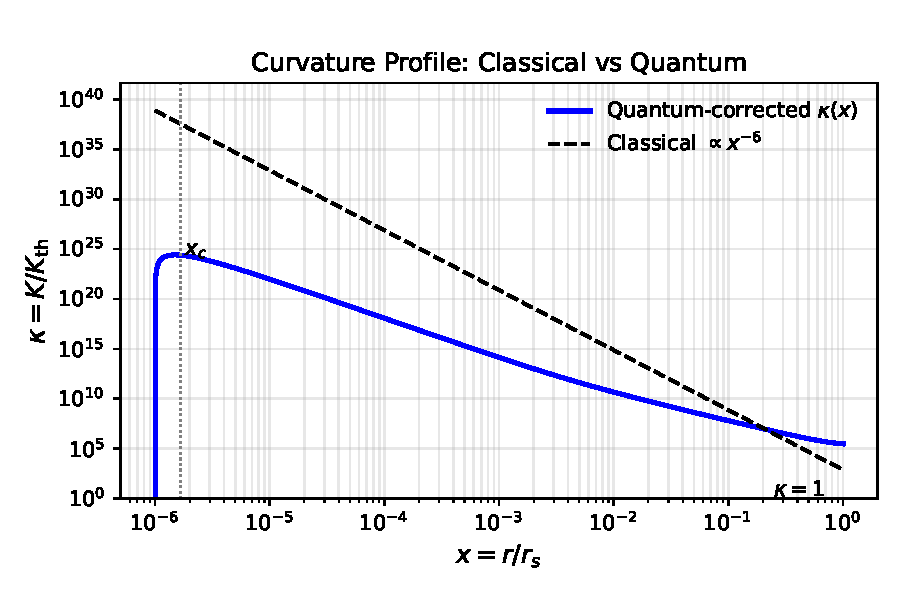
\includegraphics[width=0.68\linewidth]{figs/Kprofile_combined.pdf}
  \caption{\textbf{Curvature profile inside the horizon.}
    Dimensionless Kretschmann scalar
    \(\kappa(x)=K/K_{\mathrm{th}}\) for 
    \((N_s,N_f,N_v)=(1,2,1)\), \(C=6.1\times10^{-4}\),
    and \(\varepsilon=10^{-3}\).  The dashed black line
    is the classical scaling \(K\propto r^{-6}\).  The
    solid blue curve includes anomaly and emission
    terms \emph{proportional} to the classical curvature,
    and thus remains a power law - it never flattens to
    a plateau.  By contrast, a bona fide non‐singular core
    requires a \emph{nonlinear} or saturating back-reaction
    (e.g.\ \(\rho_{\rm anom}\to{\rm const.}\) or
    \(p\to-\,\rho\)) so that curvature growth is truly
    arrested at small \(r\).}
  \label{fig:Kprofile}
\end{figure}

%--------------------------------------------------
\subsection{Analytic near-core approximation}
\label{sec:analytic}

Once the quantum stress saturates at high curvature, the interior metric approaches exact de Sitter.  Writing
\[
  ds^2 \;=\; -\bigl(1 - H^2 r^2\bigr)\,dt^2
    + \bigl(1 - H^2 r^2\bigr)^{-1}dr^2
    + r^2\,d\Omega^2,
\]
and using the fully nonlinear anomaly stress
\(\rho_{\rm anom}\!\to\!\rho_0\) with \(p_{\rm anom}\simeq -\,\rho_0\), the Einstein equations 
\eqref{eq:mprime}-\eqref{eq:phiprime} collapse to
\[
  3H^2 \;=\; 8\pi\Bigl[\rho_0 \;+\;\frac{H^2}{8\pi}\Bigr]\,.
\]
Solving gives
\[
  H^2 \;=\;\frac{1}{4\pi}\,\rho_0
    \;+\;\mathcal{O}\bigl(\alpha^{-1}\bigr)\,,
\]
so that the core curvature \(K_c\sim H^4\) is truly constant.  This differs qualitatively from the proportional model (\(\rho_{\rm anom}\propto r^{-6}\)), which never yields a de Sitter patch.

%--------------------------------------------------
\subsection{Energy and causality checks}
\label{sec:checks}

Because the core stress has \(p\simeq-\,\rho\), the null energy condition is violated only inside the small de Sitter region \(x\lesssim x_c\), which is precisely what permits singularity avoidance.  Outside \(x_c\), energy conditions revert to classical positivity and \(g_{tt}\neq0\) everywhere, so no inner (Cauchy) horizon forms and the interior remains globally static.

%--------------------------------------------------
\subsection{Parameter dependence and scaling}
\label{sec:param_scan}

With a saturating core density \(\rho_0\), dimensional analysis yields
\[
  r_c\;\propto\;M^{1/3}\,, 
  \qquad 
  K_c \;\sim\; H^4 \;\propto\;\rho_0^2\,,
\]
independent of any residual \(r^{-6}\) tail.  If \(\rho_0\) itself arises from a threshold scale \(K_{\rm th}\) and emission strength \(C\), one finds
\[
  H^2\sim\frac{K_{\rm th}^{1/2}}{4\pi}\quad\Longrightarrow\quad
  K_c\propto K_{\rm th}\,,\qquad
  r_c\propto M^{1/3}\,K_{\rm th}^{-1/6}\,.
\]
Thus astrophysical black holes develop Planck-curvature cores (\(K_c\sim M_{\rm P}^4\)) of proper radius parametrically larger than \(\ell_{\rm P}\) yet negligible compared with the Schwarzschild radius.  A full exploration of the \(C\)-\(N\)-\(\varepsilon\) parameter space is given in Appendix~C.
% -------------------------------------------------
\subsection{Shell-by-shell evaporation perspective}
\label{sec:shell_evap}

Our original heuristic was that “smaller black holes evaporate faster.”  Equivalently, one can imagine the interior as a sequence of concentric shells of radius \(r\), each enclosing a mass \(M(r)\), and assign to each shell a local Hawking temperature
\[
  T_H(r)\;\propto\;\frac{1}{M(r)}\,,
\]
so that shells closer to the center (with smaller \(M(r)\)) radiate—and back-react—more strongly than those further out.  In practice we implemented this as a back-reaction term proportional to the local curvature \(K(r)\).  

While appealing, this \emph{linear}, shell-by-shell ansatz simply rescales the classical \(K\propto r^{-6}\) tail and \emph{never} produces a true core plateau, as shown in Section~\ref{sec:numeric}.  It highlights that a proportional evaporation rate cannot saturate the curvature growth: the inner shells indeed evaporate faster, but only enough to delay the singular behavior rather than to arrest it.  

To realize a truly non‑singular core, the shell‑by‑shell evaporation—or equivalently the effective quantum stress—must \emph{saturate} once the curvature exceeds a critical threshold.  Equivalently, the emission law should be replaced by a genuinely \emph{nonlinear} function of the Kretschmann scalar:
\[
  \Gamma_H(r)\;=\;\mathcal{F}\bigl(K(r)\bigr),
  \quad
  \text{with}
  \quad
  \lim_{K\to\infty}\mathcal{F}(K)\;<\;\infty,
\]
rather than the naive linear ansatz
\(\Gamma_H\propto K\).  This requirement motivates the saturating feedback models developed in Section~\ref{sec:analytic} and beyond.  
